\documentclass[tikz,border=8pt]{standalone}
% Shared look for every TikZ diagram. Load with \input{../../tools/tikz-style.tex}
\usepackage[T1]{fontenc}
\usepackage{lmodern}
\renewcommand{\sfdefault}{lmr}  % diagrams use the same serif as the text
\usetikzlibrary{arrows.meta, positioning, shapes.geometric, calc, fit, backgrounds}
\definecolor{cblue}{HTML}{4C78A8}
\definecolor{corange}{HTML}{F58518}
\definecolor{cgreen}{HTML}{54A24B}
\definecolor{cred}{HTML}{E45756}
\definecolor{cpurple}{HTML}{B279A2}
\definecolor{cgrey}{HTML}{6B6B6B}
\tikzset{
  every picture/.style={font=\sffamily, line width=1.2pt},
  box/.style={draw=#1, fill=#1!12, rounded corners=4pt, align=center, inner sep=7pt, minimum height=1.1cm},
  box/.default=cgrey,
  arrow/.style={-{Stealth[length=3mm]}, draw=cgrey, line width=1.4pt},
  title/.style={font=\sffamily\bfseries\Large},
  note/.style={font=\sffamily\small, text=cgrey, align=center},
}
\AtBeginDocument{\hyphenpenalty=10000 \exhyphenpenalty=10000}

\usetikzlibrary{matrix}
\begin{document}
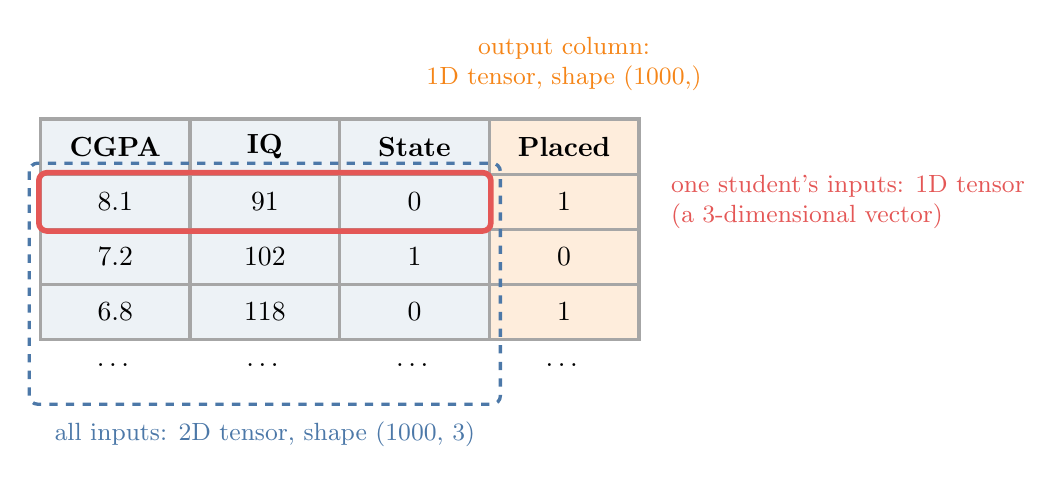
\begin{tikzpicture}
  \matrix (t) [matrix of nodes, column sep=-\pgflinewidth, row sep=-\pgflinewidth,
      nodes={minimum width=1.9cm, minimum height=0.7cm, anchor=center, draw=cgrey!60},
      row 1/.style={nodes={font=\bfseries}},
      column 1/.style={nodes={fill=cblue!10}}, column 2/.style={nodes={fill=cblue!10}}, column 3/.style={nodes={fill=cblue!10}},
      column 4/.style={nodes={fill=corange!15}}]
  { CGPA & IQ & State & Placed \\ 8.1 & 91 & 0 & 1 \\ 7.2 & 102 & 1 & 0 \\ 6.8 & 118 & 0 & 1 \\
    |[draw=none,fill=none]|\dots & |[draw=none,fill=none]|\dots & |[draw=none,fill=none]|\dots & |[draw=none,fill=none]|\dots \\ };
  \draw[cred, line width=2pt, rounded corners=3pt] (t-2-1.north west) rectangle (t-2-3.south east);
  \node[anchor=west, text=cred, align=left, font=\small] at ([xshift=0.25cm]t-2-4.east) {one student's inputs: 1D tensor\\(a 3-dimensional vector)};
  \draw[cblue, line width=1.2pt, dashed, rounded corners=3pt] ([shift={(-0.12,0.12)}]t-2-1.north west) rectangle ([shift={(0.12,-0.12)}]t-5-3.south east);
  \node[anchor=north, text=cblue, font=\small] at ([yshift=-0.2cm]t-5-2.south) {all inputs: 2D tensor, shape (1000, 3)};
  \node[anchor=south, text=corange, font=\small, align=center] at ([yshift=0.2cm]t-1-4.north) {output column:\\1D tensor, shape (1000,)};
\end{tikzpicture}
\end{document}
